\documentclass[12pt]{article}

\usepackage{hyperref}
\hypersetup{
	colorlinks,
	citecolor=blue,
	%filecolor=black,
	linkcolor=black,
	urlcolor=blue
}
\usepackage{float}
\usepackage[english]{babel}
\usepackage{natbib}
\usepackage{url}
\usepackage[utf8x]{inputenc}
\usepackage{amsmath}
\usepackage{graphicx}
\graphicspath{{images/}}
\usepackage{parskip}
\usepackage{fancyhdr}
\usepackage{vmargin}
\setmarginsrb{3 cm}{2.5 cm}{3 cm}{2.5 cm}{1 cm}{1.5 cm}{1 cm}{1.5 cm}

\title{Android Application for leasing residences}   
% Title
\author{Vassiliki Moschou, M1507 \\
	Chrysoula Themeli, M1423}                               % Author
\date{\today}                                           % Date

\makeatletter
\let\thetitle\@title
\let\theauthor\@author
\let\thedate\@date
\makeatother

\pagestyle{fancy}
\fancyhf{}
\rhead{\theauthor}
\lhead{\thetitle}
\cfoot{\thepage}

\begin{document}
	
	%%%%%%%%%%%%%%%%%%%%%%%%%%%%%%%%%%%%%%%%%%%%%%%%%%%%%%%%%%%%%%%%%%%%%%%%%%%%%%%%%%%%%%%%%
	
	\begin{titlepage}
		\centering
		\vspace*{0.5 cm}
		
\includegraphics[scale = 0.75]{ekpalogo.png}\\[1.0 cm]   % University Logo
		\textsc{\LARGE National and Kapodistrian University of Athens}\\[2.0 cm]   % University Name
		\textsc{\Large Department of Informatics and Telecommunications}\\[0.5 cm]               % Department
		\textsc{\large E-Commerce Technologies}\\[0.5 cm]               % Course Name
		\rule{\linewidth}{0.2 mm} \\[0.4 cm]
		{ \huge \bfseries \thetitle}\\
		\rule{\linewidth}{0.2 mm} \\[1.5 cm]
		
		\begin{minipage}{0.4\textwidth}
			\begin{center} \large
				\theauthor
			\end{center}
		\end{minipage}~
		\begin{minipage}{0.4\textwidth}
		\end{minipage}\\[2 cm]
		
		{\large \thedate}\\[2 cm]
		
		\vfill
		
	\end{titlepage}
	
	%%%%%%%%%%%%%%%%%%%%%%%%%%%%%%%%%%%%%%%%%%%%%%%%%%%%%%%%%%%%%%%%%%%%%%%%%%%%%%%%%%%%%%%%%
	
	\tableofcontents
	\pagebreak
	
	\listoffigures
	\listoftables
	%\lstlistoflistings
	\newpage
	
	%%%%%%%%%%%%%%%%%%%%%%%%%%%%%%%%%%%%%%%%%%%%%%%%%%%%%%%%%%%%%%%%%%%%%%%%%%%%%%%%%%%%%%%%%
	
	\section{Introduction}
	
	In order to meet the requirements of the course of E-commerce Technologies, an Android application for booking rooms/residences was implemented, following the logic of the known Airbnb application. This report includes a short definition and description of E-commerce characteristics, as well as the purpose of developing this application. There is a thorough analysis of any important decisions regarding the design process, the assumptions and all necessary details related to the project. 
	
	\subsection{Description of E-commerce}
	
	%introduction, description of e-commerce
	
	Electronic commerce (e-commerce) is a type of a business model, or a segment of a larger business model, that enables a firm or an individual to conduct business over an electronic network, typically the Internet. Electronic commerce operates in all four of the major market segments: business to business, business to consumer, consumer to consumer and consumer to business. Almost any product or service can be offered via e-commerce, from books and music to financial services and plane tickets. E-commerce has allowed firms to establish a market presence, or to enhance an existing market position, by providing a cheaper and more efficient distribution chain for their products or services.
	
	
	There are several types of electronic commerce. The most common is business to consumer, in which a business sells products or services directly to consumers over the Internet. An example of a business to consumer e-commerce transaction would be to individually purchasing a pair of sneakers through Nike's website. As of business to business type of electronic commerce, companies can sell their products or services to other companies over the Internet. An example would be the company GoDaddy, which sells domain names, websites, and hosting services to other businesses. Consumer to business electronic commerce involves consumers selling products or services to businesses. You've taken part in this form of e-commerce if you've ever completed an online payment survey where you've given your opinion about a product. Finally, regarding consumer to consumer e-commerce, consumers can sell products to other consumers via a website such as Amazon or eBay.
	
	
	The rise of e-commerce forces IT personnel to move beyond infrastructure design and maintenance and consider numerous customer-facing aspects such as consumer data privacy and security. When developing IT systems and applications to accommodate e-commerce activities, several things must be taken into consideration, like data governance related regulatory compliance mandates, personally identifiable information privacy rules and information protection protocols.
	
	Some benefits of e-commerce include its around-the-clock availability, the speed of access, the wide availability of goods and services for the consumer, easy accessibility, and international reach. Its perceived downsides include sometimes-limited customer service, consumers not being able to see or touch a product prior to purchase, and the necessitated wait time for product shipping.
	
	\subsection{Purpose of the application}
	
	As described above, e-commerce has changed the way commerce is performed for both products and services. One of the fields affected by e-commerce is tourism. Many sites and applications are implemented in order to facilitate all relevant services and transactions, like Booking, TripAdvisor, Airbnb, Trivago etc.
	
	The purpose of this project is the development of an Android Application for booking rooms/residences, enabling users to lease or rent short-term lodging including vacation rentals, apartment rentals, homestays, hostel beds, or hotel rooms. Therefore, in this application each user can have two roles. Once someone is registered, by default has the tenant (user) role. This means that he can search a residence, make a reservation, review/comment, check the inbox and send messages etc. However, there is also the ability to take over the role of host and upload information regarding residences for booking, followed by specific characteristics and availability periods. Below, the design of the database, the RESTful services and all screens of the application are described further.
	
	\section{Connection Details}
	
	\subsection{MySQL Database}
	
	For the successful initialization of the application, seven tables have been created: users, residences, rooms, reservations, reviews, conversations and messages. 
	
	\begin{itemize}
		
		\item \textbf{Users:} The fields of this table describe all necessary information for all the users registered into the application, both tenants and hosts.The mandatory fields, in order for the user to be valid, are: first name, last name, username, password and email. However, there is extra information that can be filled out later by the user. In this table, we also store the information of the role of each user (host role is enabled or not). By default host role is disabled, unless user decides to upload a residence and extend his role to host.
		\item \textbf{Residences:} In this table all the residences, entered by hosts, are described. Specifically, the information stored is: the owner, the type (house, apartment or single room), location details, short description and characteristics, cancellation policy, rules, available dates and price information of the residence. The information stored here descibes generally the residences, however it is not related to reservations, since a residence can have more than one room and different users should have the chance to book these rooms during the same period.
		\item \textbf{Rooms:} Considering the above that several users should have the opportunity to make a reservation during the same period, a table named "rooms" was created, where more specific information is contained, such as number of beds, available bathrooms and more. The field "residence\_id" connects each room with its parent residence (foreign\_key).
		\item \textbf{Reservations:} This table is used in order to store all data related to reservations that users have made. The main fields are: room\_id, tenant\_id, host\_id, period and number of guests.
		\item \textbf{Reviews:} In the application, the user can rate and comment each visited residence. Therefore, a review table is needed to keep this information.
		\item \textbf{Conversations:} An inbox service is provided to the users, where they can see messages from other users (either hosts or tenants) and reply back to them. All messages are grouped based on the subject of the conversation. As a result, two tables are created. In this table, the only necessary fields are the sender's and receiver's (user) id and the subject of the conversation.
		\item\textbf{Messages:} In addition to the above, there is the messages table with more data, such as the body of the message and a timestamp of the date in order to keep in track every action of sending/receiving and make a proper management. Moreover, the messages are linked to a conversation ("converations" table) based on the field "conversation\_id", in order for all the messages with the same subject to be grouped together.
		\item \textbf{Searches:} This table was created in order to maintain all location searches that user performs. This information is used at the home activity where application shows to user some recommendations, based on search history.
	\end{itemize}
	All above tables have a field id which is unique and auto-increment. 
	
	For our Database Model to become more clear, an Entity Relationship model was designed, showing only the most important fields of the Database, as per below:
	
	\begin{figure} [H]
		\begin{center}
			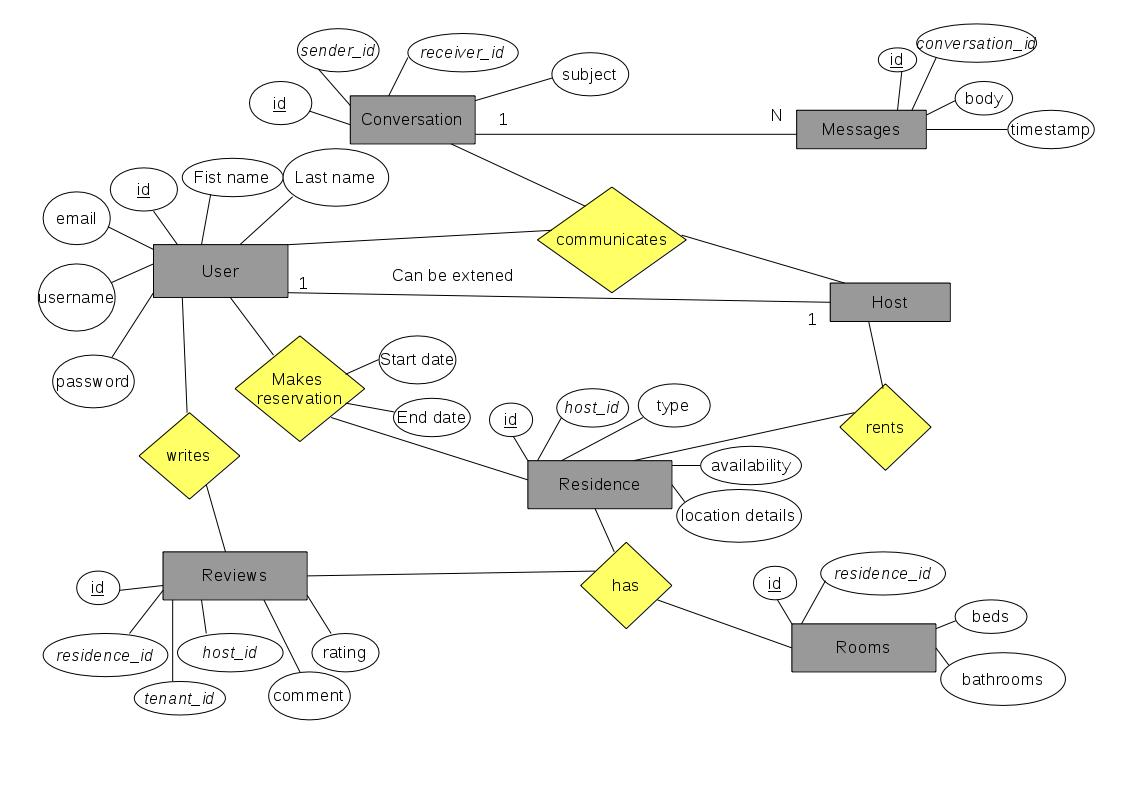
\includegraphics [scale = 0.55] {MonteloOntotitonSusxetiseon.jpg}
			\caption{Entity Relationship Model}
		\end{center}
	\end{figure}
	In above Model, all entities, their relationship and the main fields are shown. All primary keys are underlined and the foreign keys are emphasized with Italics. 
	
	Furthermore, the Enhanced Entity Relationship Model was extracted from MySQL Workbench, also showing the relations between the tables. 
	
	\begin{figure} [H]
		\begin{center}
			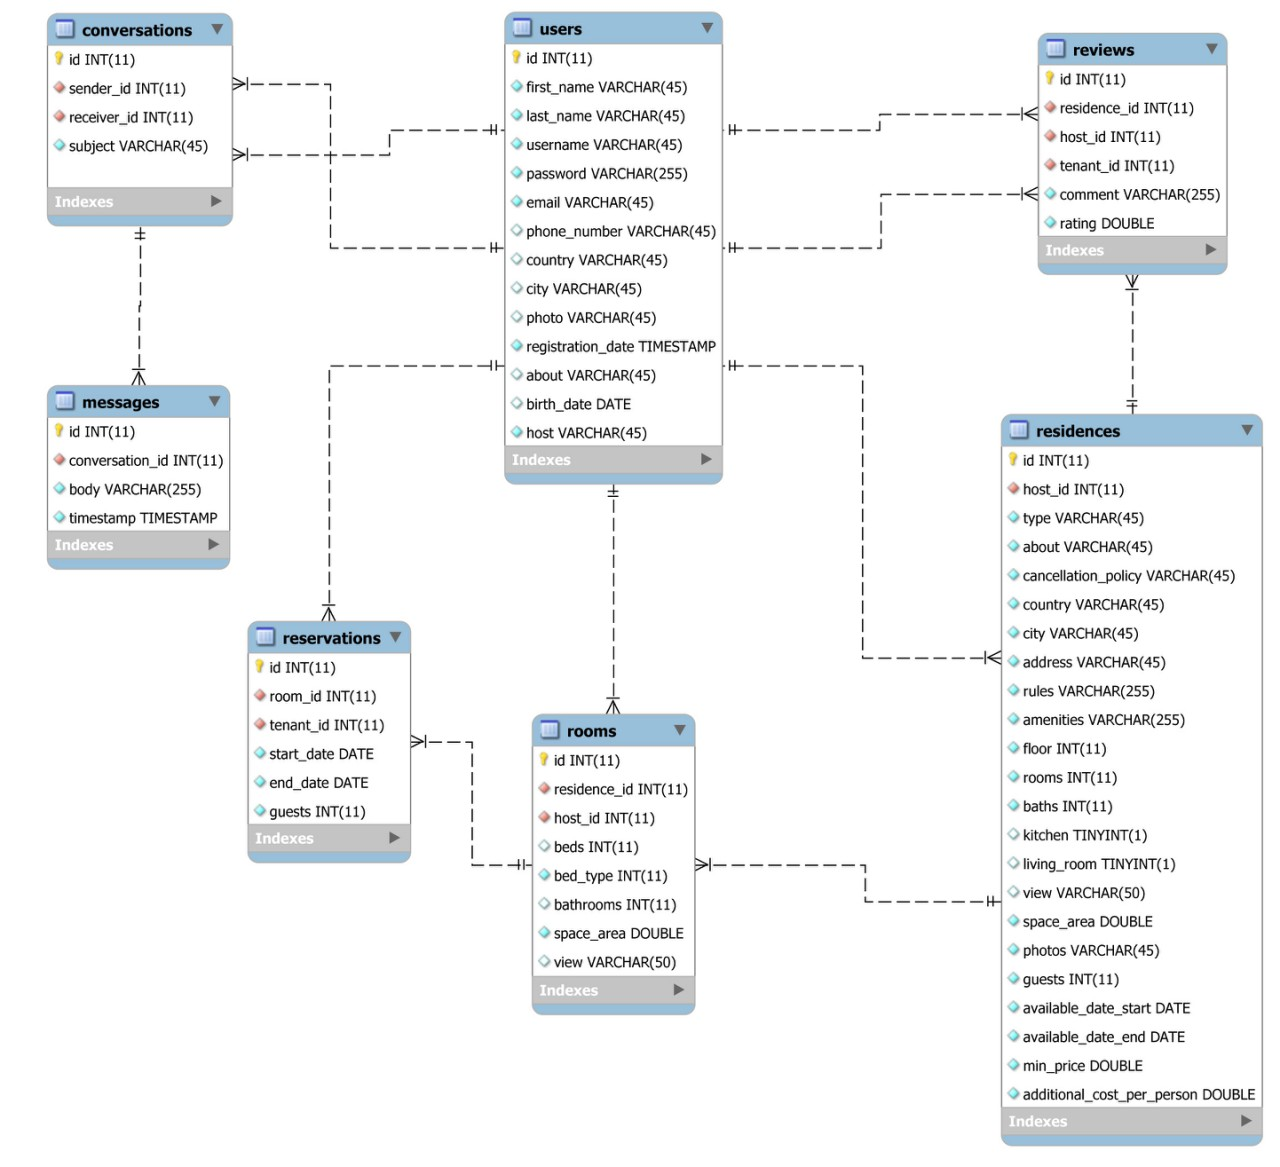
\includegraphics [scale = 0.50] {sxesiakomonetelo.jpg}
			\caption{Enhanced Entity Relationship Model}
		\end{center}
	\end{figure}
	
	
	\subsection{RESTful Services}
	The way that the application communicates with the stored information, relies absolutely to the implementation of RESTful web services. REST describes any simple interface that transmits data over a standardized interface (such as HTTP). It provides an architectural set of design rules for creating stateless services that are viewed as resources, or sources of specific information (data and functionality). Each resource can be identified by its unique Uniform Resource Identifiers (URIs). Consequently, a client (either a consumer or a business) accesses a resource using only a URI that returns the proper information needed, in a specific format that the client can handle as they want. No extra keys or credentials are required for this connection as the permissions for this access have already been set between the client and the provider of the REST service.
	
	In the world of E-commerce there is a variety of such services (like REST, SOAP or XML-RPC) that serve easily and quickly all kind of needs that clients have. For example, an e-shop can integrate several types of services into its website or application, depending always on the documentation and the standards that each service provides.
	
	Analyzing the process of an online payment, when the buyer has selected their products and proceeds to checkout, they have to fill in the credentials of their credit card in order to be confirmed as valid users. If the validation is successful, the user makes the transaction and therefore completes the checkout procedure of the product. For this operation to be handled correctly, a connection with a payment web service has already been executed (for example a physical Bank or an online Payment Service - where the latter is supported to web services too). The website doesn't have any access to the payment account credentials of each user, that's why it must connect with a Web Service, enabling the users to withdraw their money from there, and continue shopping from the website. 
	
	This procedure can be achieved with different ways, either by internal calls to the URIs of the web service through the website, or by redirection to the URIs of the Web Services that in this case, their return format, is a more user friendly environment that can guide the user to any completion steps presented. In this way, the domain of security is also supported, as each side (client and provider) has its own permissions specified, getting only the data that is considered qualified. Even the techniques used by the clients for each Web Service can vary on the permissions restrictions and the level of the risk of vulnerability from attackers.
	
	Other cases that the Web Services work on, are the known electronic malls (e-malls) that use a variety of connections of plenty e-shops and collect information of all kinds of products grouped by price, brand etc. A real case is the \textit{Skroutz} web platform which provides URIs to its' clients in order for them to send their products list externally (in an XML format for example) and manage to be visible from other sources as well.
	
	\textbf{Connection with MySQL:} For the successful operation of the RESTful Web Service, specific methods that read or write on a database must be constructed, and provide their result publicly. In more details, all the tables of the database are imported and used through MySQL queries. The desired return format that is used is JSON (could be XML, plain text, boolean, numbers etc). In practice, for viewing the list of available residences provided into the Android application, a call to the Web Service is being made, asking for the list of all the residences (that have already been added through a similar way). Next, RESTful gets triggered, and makes a connection with the database. It selects all the data from the table "residences", respecting any declared parameters or attributes, and the result (returned Array/Object/String etc) is converted to a serialized JSON value. Then it's up to the Android program to read this response, and handle it properly. Below is shown a response of a REST call that brings all the available residences from the database.
	
	%Screenshot of a sample JSON response%
	
	Something important that has to be mentioned, is the fact that the RESTful Web Service and the database should exist under the same technical environment / server, or at least under the same network. In this way, we can ensure the safety of the database, without having it open to the rest of the world and increase its vulnerability. The external client can be connected from everywhere, as it only needs a URI and the correct guidelines to make its application run.
	
	
	\section{Android Application}
	
	In this section, all screens of the application will be described, including the design decisions and the functionalities used. 
	
	Apart from that, it is important to mention here, how our Android Application consumes these RESTful Services. For this purpose, two classes have been created, the first one is called RestCallParameters class, which contains all the necessary information of a request, such as the URL, the request type (GET or POST), the return type (JSON or Plain Text) and in case of a POST request the message to be stored in the database. In addition, a class named RestCallManager is implemented. This is a different thread from main, which runs in the background, and once finished returns the JSON Object or the text from the RESTful Services.
	
	Furthermore, related to POST requests, the application should send also the user input. For this purpose, the input is stored each time to a HashMap using as a key the same name with the relevant field in the database and as value the user's input (e.g. for your reference "RegisterParameters.java"). 
	
	In order to handle GET results more efficiently, all Java classes from JPA have been created and the result from GET is retrieved as an object of these classes (Users, Residences etc). This decision has been made in order to avoid complicated containers to store all necessary information which made the code hard to understand.
	
	\subsection{Register/Log in}
	
	The first screen of our application is related to HomeActivity.java (activity\_home.xml is the relevant xml file). In this activity, it is checked whether the user is already logged in. In this case, user is welcomed at the main content of the home screen, otherwise he is redirected to the GreetingActivity.java (xml file: activity\_greeting.xml), which welcomes the user to the application and gives him the choice either to log in, if he has already an account, or to register. This is handled with the SharedPreferences. When a user logs in or registers, the relevant username is stored to the SharedPreferences and passed to home and next activities. In addition, this information is added to onResume  and onRestart, therefore user is always logged in when enters the application. In the footer of home activity, there is a log out button, which clears the SharedPreferences and when user presses it, he is redirected to GreetingActivity.
	
	%TLS and image upload to be completed
	When the user clicks on the Register button at the GreetingActivity, a new screen appears (RegisterActivity.java and activity\_register.xml) with mandatory fields to be completed by them. The fields are: first name, last name, email, username, password and confirm password. Our application, checks if all the fields are completed and also whether the password and confirmation password are identical. Furthermore, two GET requests are used to check separately email and username. In case one of these fields are found in the DataBase, application does not let the user to proceed and asks him to refill correctly either email or username field. 
	
	Finally, once the form is completed correctly, when the user presses register button, a POST request is sent to the database, in order to store the data to respective table. In order to send the POST request, android application creates a JSON Object and provides it to the RESTful services. A boolean variable is used to check the result of POST request. If the request was successful, user proceeds to the Home screen.
	
	On the other hand, when user clicks the Login button, the relevant form appears and asks him to fill in the username and the password(LoginActivity and activity\_login). Following a similar logic to the above process, a GET request is sent in order to check if username and password are correct. For this purpose, respective query and method in RESTful services have been created. If user inserts wrong details(based on the comparison between user input and GET result) a message appears and fields should be filled again, otherwise the home screen appears and user now is logged in.
	
	\subsection{Home Page}
	In this activity, it is checked if user is logged in, if not the application is redirected to the Greeting Activity as mentioned above. Otherwise, user can see the home page, where a search field is located on the top of the screen. Below, a list of recommendations is presented to user, based on his search activity (if user is new the most popular residences appear).
	%Session, SharedPreferences
	In order to keep user logged in, SharedPreferences are passed to the HomeActivity's methods onCreate, onResume and onRestart. Method on BackPressed, if user is logged in, does not let him go back to login screen and restarts the HomeActivity. At the bottom of this activity, a footer appears with buttons that let the user enter to his inbox, edit his profile, switch to another role and log out from the application.
	
	At the top of the home screen, there is a search field that lets user to search residences entering the city and period he wants. This function will be described further to the next section (Search).
	
	Moreover, method popularRecommendations implemented so as to get recommended residences and show them when HomeActivity starts. In popularRecommendations, username is passed as argument and based on this data application retrieves also the userId. All calls are performed from RestCalls(package util), in this case getUserId was called. Based on userId, it is checked if user has performed any searches yet. A GET request is sent using method getSearchedCities and the result is stored to a Set (relevantCity). If set's size is zero, user has not searched anything yet, therefore most popular residences appears as recommendation. Method getReviews is called and the result is stored to an ArrayList of Reviews. From this object, respective residences are stored to reviewedResidences (ArrayList of Residences). On the other hand, cities stored in the set are checked one by one and all residences in these cities are stored in reviewedResidences. After having all necessary residences, duplicates are removed from ArrayList (using Set hs), since from the first case (get residences based on reviews) we may have stored the same residence many times (many reviews may be related to a residence).
	
	Having the reviewedResidences, we can now get the related Rooms and Reviews for each residence. This information can be stored to this object (reviewedResidences), since class Residences has two collections (for Rooms and Reviews). Reviews are needed in order to sort the Residences based on rating (calculating the average rating). In Residences class, a compareTo method, compares two Residences based on their average rating (getAverageRating method). Finally, sorted residences are passed to the onCreate method as result. In order to show the results to user, a listview layout was implemented. Each list item shows the representative photo of a residence, its price, the city and the price. An adapter (CustomListAdapter) was used so as to create the list items.
	
	\subsection{Search}
	
	\subsection{Detailed presentation of residences}
	\subsection{Inbox}
	\subsection{Reviews}
	\subsection{User profile}
	\subsection{Host Role and new residence upload}
	
	
	\bibliographystyle{plain}
	\bibliography{biblist}
	
	\begin{itemize}
		\item \emph{MySQL}
		\begin{itemize}
			\item 
		\end{itemize}
		\item \emph{RESTful Services}
		\begin{itemize}
			\item https://netbeans.org/kb/docs/websvc/rest.html
			\item https://docs.oracle.com/cd/E24329\_01/web.1211/e24983/overview.htm
			\item http://www.naun.org/main/NAUN/computers/16-579.pdf
			\item https://spring.io/guides/gs/consuming-rest-android/
		\end{itemize}
		\item \emph{Android Development}
		\begin{itemize}
			\item https://developer.android.com/reference/android/os/AsyncTask.html
			\item https://developer.android.com/training/volley/index.html
		\end{itemize}
	\end{itemize}
	
\end{document}